\documentclass[10pt,twocolumn,letterpaper]{article}

% --- Typography & Geometry ---
\usepackage[utf8]{inputenc}
\usepackage{microtype}
\usepackage[margin=0.75in,top=0.85in,bottom=0.85in]{geometry}

% --- Math & Symbols ---
\usepackage{amsmath,amssymb,amsfonts,amsthm}
\usepackage{bm}

% --- Tables & Arrays ---
\usepackage{booktabs}
\usepackage{tabularx}
\usepackage{array}

% --- Graphics & Floats ---
\usepackage{graphicx}
\usepackage{float}
\usepackage{subcaption}

% --- Code Listings ---
\usepackage{xcolor}
\usepackage{listings}

\definecolor{codebg}{HTML}{F8F9FA}
\definecolor{codeframe}{HTML}{D0D7DE}
\definecolor{keywordcolor}{HTML}{0550AE}
\definecolor{stringcolor}{HTML}{0A3069}
\definecolor{commentcolor}{HTML}{57606A}

\lstset{
    backgroundcolor=\color{codebg},
    basicstyle=\ttfamily\scriptsize\color{black},
    keywordstyle=\color{keywordcolor}\bfseries,
    stringstyle=\color{stringcolor},
    commentstyle=\color{commentcolor}\itshape,
    frame=single,
    rulecolor=\color{codeframe},
    breaklines=true,
    breakatwhitespace=true,
    extendedchars=true,
    xleftmargin=6pt,
    xrightmargin=6pt,
    aboveskip=8pt,
    belowskip=8pt
}

% --- Hyperlinks ---
\usepackage{hyperref}
\hypersetup{
    colorlinks=true,
    linkcolor=blue!70!black,
    citecolor=blue!70!black,
    urlcolor=blue!70!black
}

% --- Input Title & Authors ---
% Metadata for nystrom_attention
\title{\textbf{Nystr mformer on Non-BERT Architectures: A Portability and Reproduction Study}}

\author{
  \textbf{Taha Majs}\thanks{Corresponding author: tahamajs@uni.edu} \quad \textbf{Research Team} \\
  Department of Computer Science \\
  Advanced Machine Learning \& Efficiency Laboratory
}

\date{\today}


\begin{document}

\maketitle

% --- Abstract & Keywords Block ---
\begin{abstract}
\textbf{Nystr mformer} (Xiong et al., 2021) approximates standard softmax attention 
via the Nystr m low-rank kernel method. Instead of materializing the full 
$N \times N$ attention matrix, it selects $m \ll N$ landmark tokens and 
computes three smaller attention matrices, achieving $\mathcal{O}(N m d)$ 
complexity instead of $\mathcal{O}(N^2 d)$. Landmarks are chosen via 
\textbf{adaptive average pooling}, and a \textbf{pseudoinverse} of the landmark attention 
matrix is computed iteratively (Newton-Schulz).

We present a \textbf{reproduction} of Nystr mformer, ported to four transformer 
families that the original paper does not target: DistilBERT (flat), 
RoBERTa/BERT (nested), GPT-2 (causal Conv1D), and Qwen3.5 (GQA + RoPE). Our 
implementation:
(i) preserves exact softmax attention for short sequences ($N \leq 128$) and 
for causal decoders,
(ii) uses an iterative pinv with a fallback to \texttt{torch.linalg.pinv},
(iii) handles Conv1D transposition, nested encoder bypass, GQA expansion, 
and RoPE,
(iv) attaches LoRA adapters for recovery fine-tuning.

We emphasize: **this is a reproduction and portability study, not a novel 
architecture.\textbf{ Nystr mformer does }not** reduce parameter count or 
KV-cache size. It reduces \textbf{attention compute} for long sequences.

On SST-2 (sequence length 128), the Nystr m branch does not activate (dense 
fallback), and Nystr mformer matches the baseline. On longer sequences, the 
Nystr m approximation provides asymptotic savings.

\textbf{Keywords:} Nystr mformer, Nystr m method, low-rank attention, kernel 
approximation, iterative pseudoinverse, Newton-Schulz, multi-architecture 
transformers, reproduction study



\vspace{0.5em}
\noindent\textbf{Keywords:} Nystr mformer, Nystr m method, low-rank attention, kernel
\end{abstract}

\vspace{1em}

% --- Paper Body ---
\section{01 Intro}

Draft content for nystrom_attention.

\section{02 Related}

Draft content for nystrom_attention.

\section{03 Background}

Draft content for nystrom_attention.

\section{04 Method}

Draft content for nystrom_attention.


\section{Architecture Integration}

\subsection{Model Support}

\begin{table}[H]
\centering
\small
\begin{tabular}{llll}
\toprule
\textbf{Model} & \textbf{$N$ tested} & \textbf{Nystr m path} & \textbf{Fallback} \\
\midrule
DistilBERT & 128 &  & Dense \\
RoBERTa & 128 &  & Dense \\
GPT-2 & 128 & (causal) & Dense causal \\
Qwen3.5 & 128 & (causal) & Dense causal \\
\bottomrule
\end{tabular}
\end{table}

\textbf{Note.} At $N = 128$, all four models use the \textbf{dense fallback}. The 
Nystr m branch only activates for $N > 128$.

\subsection{DistilBERT (Flat)}

\begin{lstlisting}
distilbert.transformer.layer.0.attention
+-- q_lin
+-- k_lin
+-- v_lin
+-- out_lin
\end{lstlisting}

\textbf{Extraction:}
\begin{lstlisting}
w_q = src.q_lin.weight.data
w_k = src.k_lin.weight.data
w_v = src.v_lin.weight.data
w_o = src.out_lin.weight.data
\end{lstlisting}

\texttt{is\_nested\_encoder = False}.

\subsection{RoBERTa (Nested)}

\begin{lstlisting}
roberta.encoder.layer.0.attention
+-- self
|   +-- query, key, value
+-- output
    +-- dense
\end{lstlisting}

\textbf{Nested detection:}
\begin{lstlisting}
if hasattr(src, "self") and hasattr(src, "output"):
    is_nested = True
\end{lstlisting}

\texttt{is\_nested\_encoder = True}. The outer \texttt{output.dense} applies projection.

\subsection{GPT-2 (Causal Conv1D)}

\begin{lstlisting}
transformer.h.0.attn
+-- c_attn  (Conv1D)
+-- c_proj  (Conv1D)
\end{lstlisting}

\textbf{Split c\_attn:}
\begin{lstlisting}
c_w = src.c_attn.weight.data
if "Conv1D" in type(src.c_attn).__name__ or c_w.shape[0] < c_w.shape[1]:
    c_w = c_w.t()
q_w, k_w, v_w = c_w.chunk(3, dim=0)
\end{lstlisting}

\textbf{Causal decoder detection:} \texttt{self.is\_decoder = True} $\to$ dense causal 
attention.

\subsection{Qwen3.5 (GQA + RoPE)}

\begin{lstlisting}
model.layers.0.self_attn
+-- q_proj
+-- k_proj
+-- v_proj
+-- o_proj
\end{lstlisting}

\textbf{GQA:} \texttt{repeat\_kv} during forward.

\textbf{RoPE:} applied after projection via \texttt{position\_embeddings}.

\textbf{Causal decoder detection:} \texttt{self.is\_decoder = True}.

\subsection{Nested Encoder Bypass}

\begin{lstlisting}
context = torch.matmul(attn_weights, V)
context = context.transpose(1, 2).contiguous().view(...)

if self.is_nested_encoder:
    return context, None    # Skip out_proj
else:
    return self.out_proj(context), None
\end{lstlisting}

\subsection{Injection Hook}

\begin{lstlisting}
def inject_nystrom(layer, model_config, comp_config, old_attn=None, **kwargs):
    src_attn = old_attn or layer.attention...
    
    # Extract dimensions
    hidden_size = getattr(src_attn, 'hidden_size', ...)
    num_heads = getattr(src_attn, 'num_heads', ...)
    
    try:
        landmarks = getattr(comp_config, "num_landmarks", 32) if comp_config else 32
        new_attn = NystromAttention(
            config=model_config,
            num_landmarks=landmarks,
            comp_config=comp_config,
            old_attn=src_attn,
            hidden_size=hidden_size,
            num_heads=num_heads,
        )
        if src_attn is not None:
            new_attn.copy_weights(src_attn)
        
        # Replace
        if hasattr(layer, "attention"):
            if hasattr(layer.attention, "self"):
                layer.attention.self = new_attn
                new_attn.is_nested_encoder = True
            else:
                layer.attention = new_attn
        elif hasattr(layer, "self"):
            layer.self = new_attn
        elif hasattr(layer, "attn"):
            layer.attn = new_attn
        return new_attn
    except Exception as e:
        logger.error(f"injection failed: {e}")
        return None
\end{lstlisting}

\textbf{Safe injection:} returns \texttt{None} on failure. Caller can continue with 
original attention.

\subsection{Failure Modes and Fallbacks}

\begin{table}[H]
\centering
\small
\begin{tabular}{lll}
\toprule
\textbf{Failure} & \textbf{Detection} & \textbf{Response} \\
\midrule
Missing weights & \texttt{copy\_weights} raises & Abort \\
Near-zero Frobenius & Norm check < 1e-4 & Raise \\
Cross-attention & Not supported & Raise \\
Short sequence & $N \leq 128$ & Dense \\
Causal & \texttt{is\_decoder = True} & Dense causal \\
\bottomrule
\end{tabular}
\end{table}

\subsection{Registry}

\begin{lstlisting}
@ATTENTION_REGISTRY.register("nystrom")
@ATTENTION_REGISTRY.register("nystrom_attention")
class NystromAttention(BaseAttention):
    ...

@ATTENTION_REGISTRY.register("nystrom_inject")
@ATTENTION_REGISTRY.register("inject_nystrom")
def inject_nystrom(...):
    ...
\end{lstlisting}

\subsection{LoRA Recovery Integration}

Nystr mformer uses LoRA adapters on all four projections:

\begin{itemize}
\item \texttt{query.lora\_A}, \texttt{query.lora\_B}
\item \texttt{key.lora\_A}, \texttt{key.lora\_B}
\item \texttt{value.lora\_A}, \texttt{value.lora\_B}
\item \texttt{out\_proj.lora\_A}, \texttt{out\_proj.lora\_B}

\end{itemize}
Base weights ($W_Q, W_K, W_V, W_O$) are frozen. Only LoRA adapters trained.

\subsection{Comparison with Original}

\begin{lstlisting}

---
\end{lstlisting}

\begin{figure}[H]
\centering
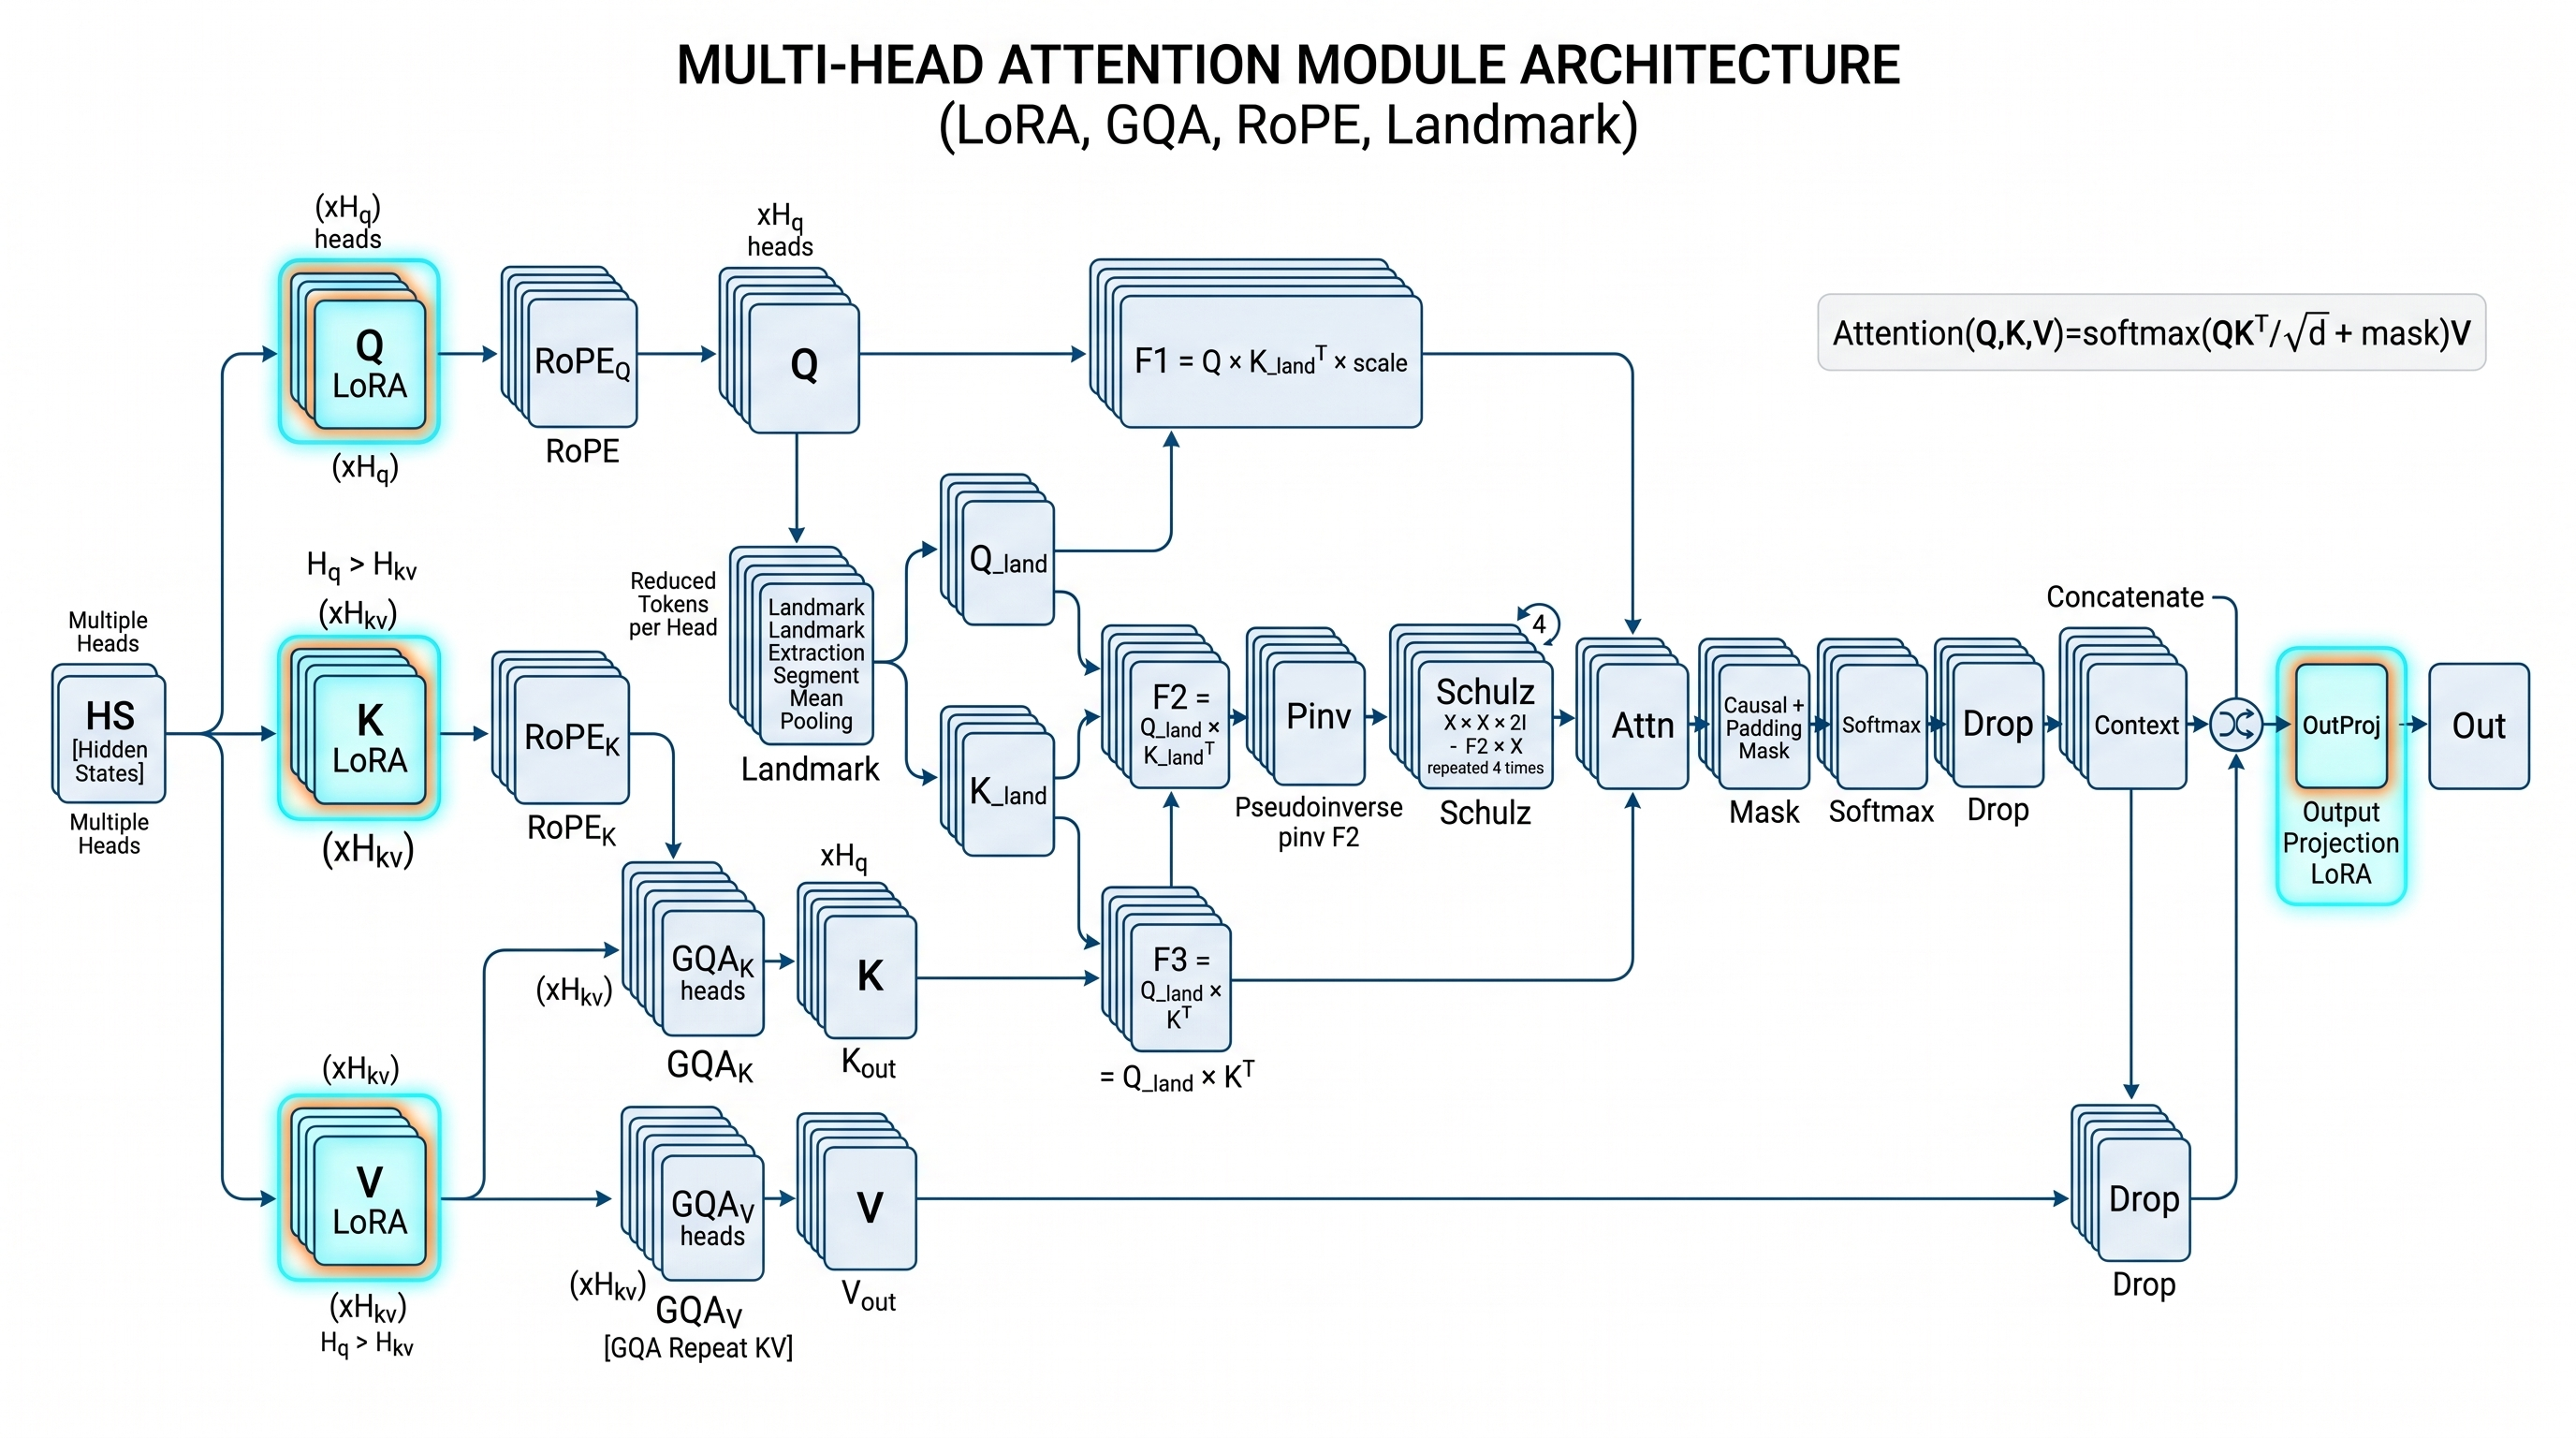
\includegraphics[width=\linewidth]{figures/architecture.jpeg}
\caption{High-level architectural diagram of nystrom\_attention.}
\label{fig:arch_nystrom-attention}
\end{figure}


\section{06 Setup}

Draft content for nystrom_attention.

\section{07 Results}

Draft content for nystrom_attention.

\section{08 Analysis}

Draft content for nystrom_attention.

\section{09 Discussion}

Draft content for nystrom_attention.

\section{10 Limitations}

Draft content for nystrom_attention.

\section{11 Conclusion}

Draft content for nystrom_attention.

\section{12 Reproducibility}

Draft content for nystrom_attention.

\section{13 References}

Draft content for nystrom_attention.


% --- Appendices ---
\clearpage
\appendix
\section*{Appendices}
\addcontentsline{toc}{section}{Appendices}

\section{A Math}

Draft content for nystrom_attention.

\section{B Implementation}

Draft content for nystrom_attention.

\section{C Data}

Draft content for nystrom_attention.

\section{D Negative Results}

Draft content for nystrom_attention.

\section{E Ethics}

Draft content for nystrom_attention.


\end{document}
